\documentclass{article}
\usepackage[utf8]{inputenc}
\usepackage{polski}
\usepackage{geometry}
\usepackage{mathabx}
\usepackage{tikz}
\usepackage{amsmath}
\usepackage{graphicx}
\usepackage{subfig}
\usepackage{amsmath}
\usepackage{hyperref}
\usepackage{pdfpages}
\usepackage{siunitx}

\geometry{
a4paper,
total={170mm,257mm},
left=20mm,
top=20mm
}
\renewcommand\thesection{}

\title{Podstawy baz danych\\ Projekt konferencje}
\author{Agnieszka Dutka, Maciek Trątnowiecki}
\date{AGH, Styczeń 2020}

\begin{document}
\maketitle
\section{Objaśnienie schematu bazy}
        \begin{itemize}
            \item Clients - Reprezentuje klientów chcących opłacić miejsca na konferencjach i warsztatach. Klientem może być zarówno firma, jak i osoba prywatna. W zależności od tego dane klienta reprezentowane są przez odpowiednią relację w bazie. 
            
            \item Companies - Jeśli klient jest firmą, przechowuje jego dane. 
            
            \item Participants - Jeśli klient jest osobą prywatną, przechowuje jego dane.
            
            \item Conferences - Reprezentuje konferencję z którą powiązane są odpowiednie dni konferencyjne, oraz warsztaty. 
            
            \item Conference\_days - Reprezentuje pojedynczy dzień konferencji. Powiązana jest z nim ustalona opłata za uczestnictwo. Zniżki obowiązujące w zależności od daty rejestracji zwarte są w relacji Early\_Signup\_Discounts. 
            
            \item Early\_Signup\_Discounts - Odpowiada za informację o tabeli zniżek na dany dzień konferencyjny. Pojedyncza zniżka przechowywana jest w krotce z atrybutami w postaci procentowej obniżki ceny standardowej, oraz ostatniego dnia w którym obowiązuje. 
            
            \item Conference\_day\_reservations - Realizuje rezerwacje na poszczególny dzień konferencji. Każda rezerwacja powiązana jest z klientem, który ją opłaca. Za powiązanie rezerwacji z uczestnikiem odpowiada osobna relacja. Zawiera także pole due\_price określające termin płatności. Atrybut active odpowiada za możliwość rezygnacji z podjętej rezerwacji (uznaliśmy, że usuwanie krotki z bazy może nie być optymalnym rozwiązaniem, jako że zawarte w niej dane mogą jeszcze być przydatne z punktu widzenia logiki biznesowej). Atrybuty adult\_seats i student\_seats służą do liczenia kosztu podjęcia rezerwacji przed powiązaniem jej z uczestnikami konferencji. 
            
            \item Conference\_day\_registration - Wiąże rezerwację z uczestnikami konferencji. Atrybut is\_student informuje, czy danemu uczestnikowi przysługuje zniżka studencka. 
            
            \item Payments - Przechowuje informacje o wpływach pieniężnych powiązanych z daną rejestracją. 
            
            \item Workshops - Reprezentuje warsztaty odbywające się w trakcie odpowiednich dni konferencyjnych.
            
            \item Workshops\_reservations - Opisuje rezerwacje na warsztaty w sposób analogiczny do rezerwacji na konferencje. 
            
            \item Workshops\_registrations - Łączy rezerwację z uczestnikami w sposób analogiczny do dni konferencyjnych.
            
        \end{itemize}
    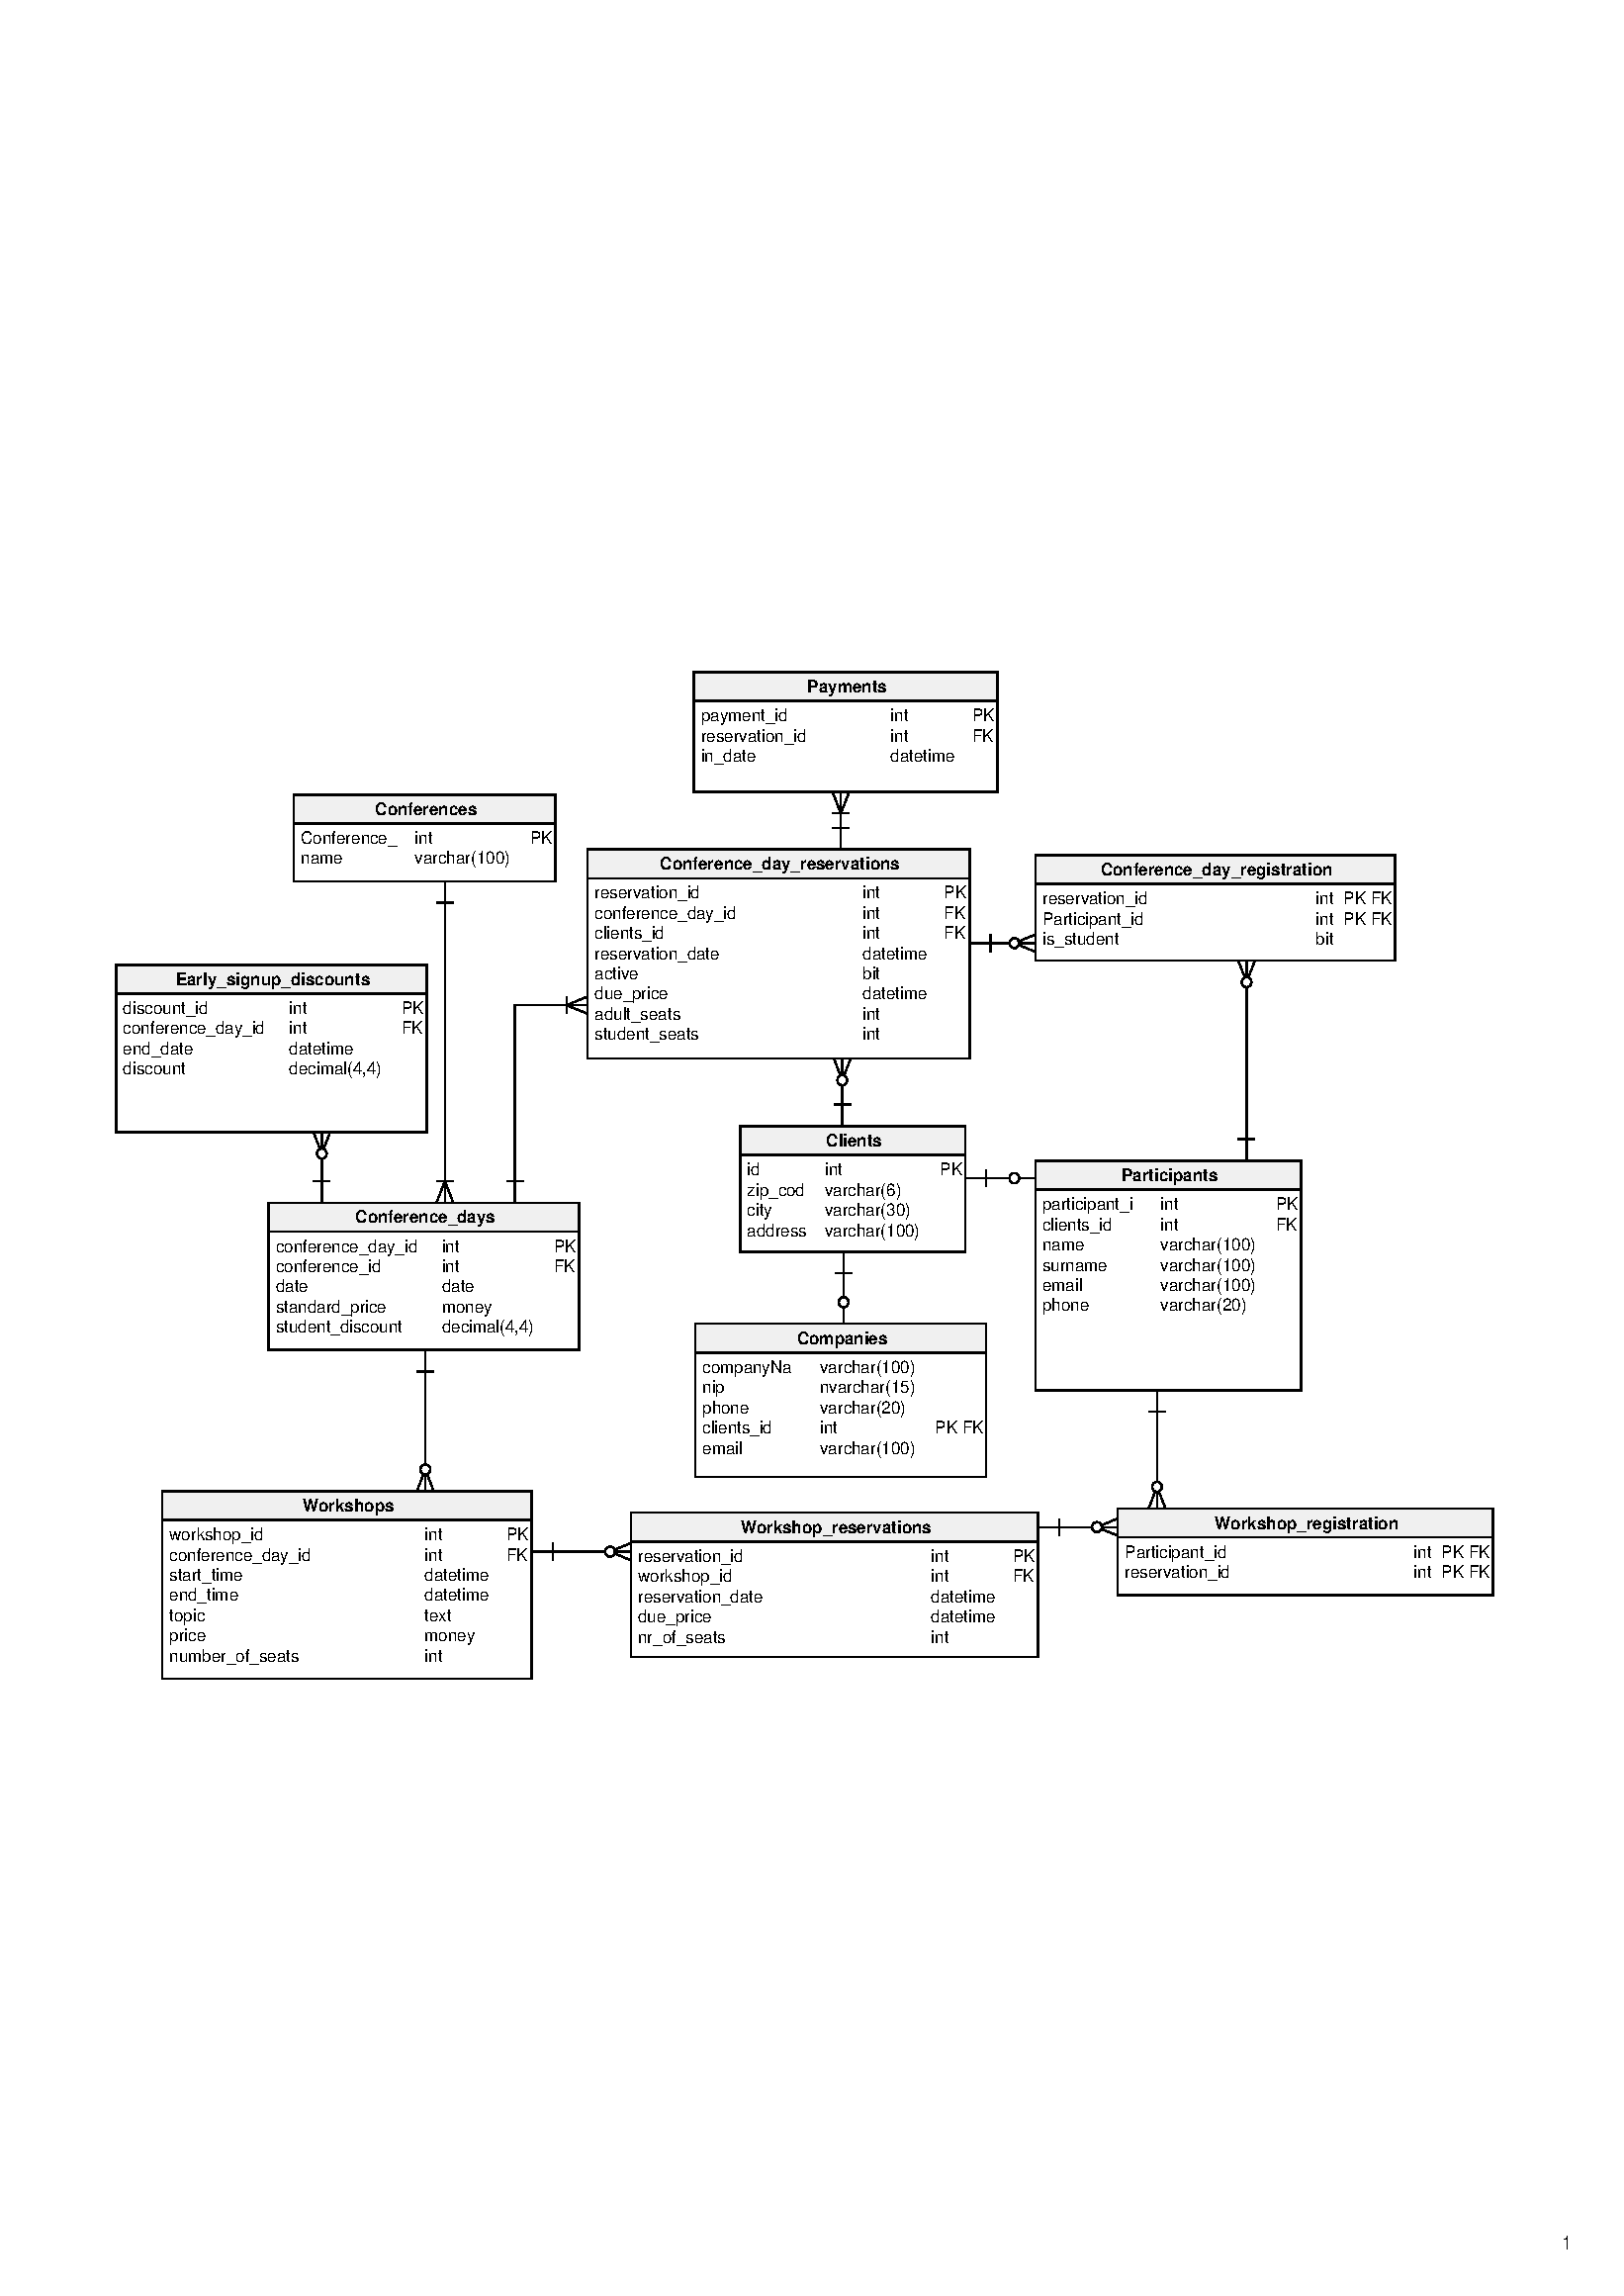
\includepdf{../Diagrams/Scheme.pdf}    
\end{document}